\chapter[Evaluation]{Evaluation}
\label{Chap:Evaluation}
% ***************************************************
%Evaluation 
% ***************************************************

\section{Raw Performance Benchmarks}
Here, the different configurations of VexRiscv: single-core, dual-core and quad core; will be compared in terms of performance alongside the Raspberry Pi Model 4B 1GB. For each one, we will run the performance benchmark, \textit{stress-ng}, which profiles the IO overhead and memory usage of multiple cores, along with \textit{Iperf3}, to gauge ethernet throughput capabilities.

\subsection{Iperf3}
As ethernet is a vital component of the application, it makes sense to evaluate the capabilities of the link, especially the average bitrate we can expect. After running \texttt{iperf3 -s}, which sets the device as a server and listens, another Raspberry Pi was chosen from the cluster to act as a client via running:
\begin{verbatim}    
iperf3 -c 192.168.1.50 -t 30 -i 1 -w 8K -P 1 -R
\end{verbatim}
This begins a single-threaded (\texttt{-P 1}), client that sends and receives TCP transmissions to \textit{192.168.1.50}, for 30 seconds, sampling the bitrate every second (\texttt{-i 1}). Most notably, it constrains the TCP window size (\texttt{-w 8K}), to 8Kb, which matches the current size of the board's TX or RX ethernet buffers, more closely resembling the stop-start transfers in our software setup. Here are the results:

\begin{table*}[ht]
    \centering
    \caption{Ethernet Throughput Comparison of Configurations}
    \label{table:ethernet1}
    \begin{tabular}{lllll}
                                & \multicolumn{3}{l}{VexRiscvSMP, 100MHz} & RPi    \\ \cline{2-5} 
                                & Single        & Dual       & Quad       & 4B 1GB \\ \hline
    Amount Transferred (MB)     & 31.5          & 35.5       & 42.0       & 1.13k  \\
    Amount Recieved (MB)        & 31.4          & 35.4       & 41.9       & 1.13k  \\
    Sending Bitrate (MBits/s)   & 8.78          & 9.90       & 11.7       & 323    \\
    Receiving Bitrate (MBits/s) & 8.77          & 9.89       & 11.7       & 323    \\
    TCP Retransmissions         & 0             & 0          & 1          & 0      \\ \hline
    \end{tabular}
\end{table*}

It is clear that the gigabit ethernet capabilities of the Raspberry Pi far outweigh the ethernet capabilities of the board, achieving 26x more throughput than that of the quad-core VexRiscvSMP. Keep in mind as well, the Raspberry Pi is throttled because of the 8Kb window size we set. Additionally, the core amount does have an effect on the bitrate as the quad core is 1.8MBits/s faster than the dual core, which is 1.12MBits/s faster than the single core. However, an overall improvement of 32\% across cores is basically negligible since the absolute performance is still far below what is required for what is essentially a high-speed ethernet application. It is clear from this benchmark alone that the bitrate will be a significant bottleneck for the design.

\subsection{Stress NG}
Stress-ng is a versatile benchmarking tool designed to stress test various components of a CPU. The command:
\begin{verbatim}
stress-ng --cpu $CORE_COUNT --io 2 --vm 1 --vm-bytes 128M --timeout 60s 
--metrics-brief
\end{verbatim}
Runs a set of tests in parallel. The rest of the arguments determine the amount of tests and the type: \texttt{--cpu}, creates CPU-intensive tasks equal to the core count; \texttt{--io}, creates two I/O-intensive tasks; and \texttt{--vm}, allocates and uses 128MB of virtual memory. This will evaluate for us how the system performs under combined CPU, I/O, and memory pressure, as well as how these metrics vary with the amount of cores. Additionally, the test will timeout after 60 seconds or until $6\cdot$\texttt{\$CORE\_COUNT} CPU bogo ops have been completed. Here are the results:

\begin{table*}[ht]
    \centering
    \caption{Stress-ng Comparison of Configurations}
    \label{table:stress1}
    \begin{tabular}{lllll}
                                  & \multicolumn{3}{l}{VexRiscvSMP, 100MHz} & RPi       \\ \cline{2-5} 
                                  & Single      & Dual        & Quad        & 4B 1GB    \\ \hline
    CPU bogo ops                  & 6           & 12          & 24          & 12,483    \\ \hline
    CPU real time (s)             & 125.34      & 119.09      & 121.30      & 60.03     \\
    CPU usr time (s)              & 78.32       & 164.00      & 378.16      & 146.85    \\
    CPU sys time (s)              & 0.01        & 0.12        & 0.09        & 0.03      \\
    CPU bogo ops/s (real time)    & 0.05        & 0.10        & 0.20        & 207.94    \\
    CPU bogo ops/s (usr+sys time) & 0.08        & 0.07        & 0.06        & 84.99     \\ \hline
    IO bogo ops                   & 21,794      & 31,190      & 27,819      & 440,066   \\ \hline
    IO real time (s)              & 60.00       & 60.01       & 60.00       & 60.00     \\
    IO usr time (s)               & 2.74        & 3.56        & 3.42        & 10.34     \\
    IO sys time (s)               & 25.71       & 44.44       & 66.44       & 48.56     \\
    IO bogo ops/s (real time)     & 363.22      & 519.76      & 463.65      & 7,334.31  \\
    IO bogo ops/s (usr+sys time)  & 766.05      & 649.79      & 398.21      & 7,472.11  \\ \hline
    VM bogo ops                   & 2,280       & 3,053       & 2,464       & 617,668   \\ \hline
    VM real time (s)              & 61.92       & 62.54       & 61.54       & 60.16     \\
    VM usr time (s)               & 7.57        & 10.72       & 18.10       & 27.27     \\
    VM sys time (s)               & 7.60        & 14.93       & 18.32       & 6.78      \\
    VM bogo ops/s (real time)     & 36.82       & 48.82       & 40.04       & 10,266.29 \\
    VM bogo ops/s (usr+sys time)  & 150.30      & 119.03      & 67.66       & 18,143.58 \\ \hline
    Total time taken (s)          & 125.45      & 120.31      & 122.76      & 60.00     \\ \hline
    \end{tabular}
\end{table*}
\raggedbottom

\begin{figure*}[ht]
    \centering
    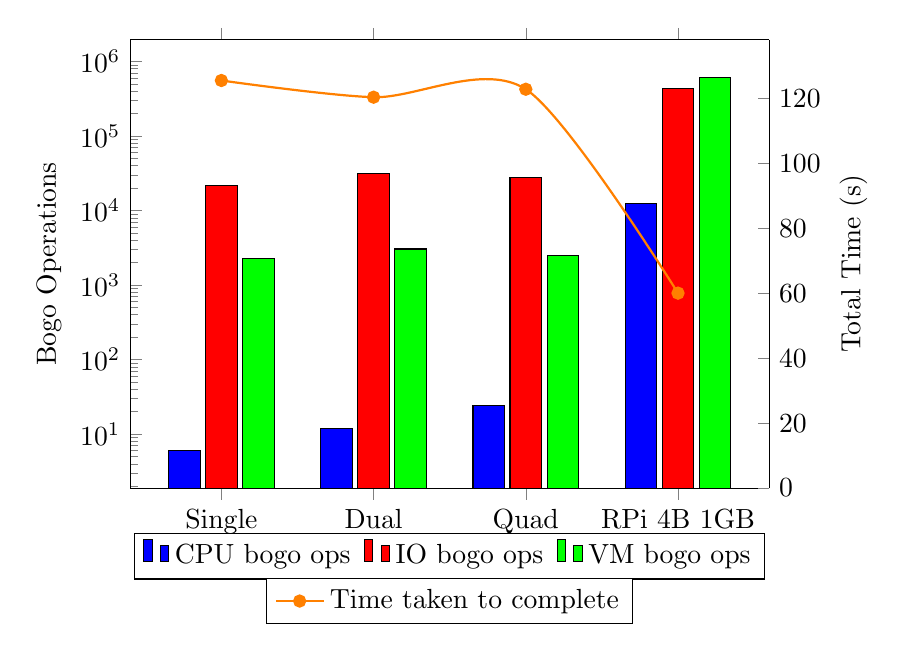
\begin{tikzpicture}
    \begin{axis}[
        width=0.8\textwidth,
        height=0.6\textwidth,
        ybar,
        bar width=0.4cm,
        enlarge x limits=0.2,
        legend style={
            at={(0.5, -0.1)},
            anchor=north,
            legend columns=-1,
            /tikz/every even column/.append style={column sep=0.1cm}
        },
        ylabel={Bogo Operations},
        symbolic x coords={Single, Dual, Quad, RPi 4B 1GB},
        xtick=data,
        axis y line*=left,
        ylabel near ticks,
        ymode=log,
        log origin=infty,
        ]
    \addplot[fill=blue] coordinates {
        (Single,6) (Dual,12) (Quad,24) (RPi 4B 1GB,12483)};
    \addplot[fill=red] coordinates {
        (Single,21794) (Dual,31190) (Quad,27819) (RPi 4B 1GB,440066)};
    \addplot[fill=green] coordinates {
        (Single,2280) (Dual,3053) (Quad,2464) (RPi 4B 1GB,617668)};
    \addlegendentry{CPU bogo ops}
    \addlegendentry{IO bogo ops}
    \addlegendentry{VM bogo ops}
    \end{axis}
    
    \begin{axis}[
        width=0.8\textwidth,
        height=0.6\textwidth,
        enlarge x limits=0.2,
        legend style={
            at={(0.5,-0.2)},
            anchor=north,
            legend columns=-1,
            /tikz/every even column/.append style={column sep=0.5cm}
        },
        axis y line*=right,
        axis x line=none,
        ylabel={Total Time (s)},
        ylabel near ticks,
        ymin=0,
        symbolic x coords={Single, Dual, Quad, RPi 4B 1GB},
        ]
    \addplot[smooth, thick, orange, mark=*] coordinates {
        (Single,125.45) (Dual,120.31) (Quad,122.76) (RPi 4B 1GB,60.00)};
    \addlegendentry{Time taken to complete}
    \end{axis}
    \end{tikzpicture}
    \caption{Stress-ng Performance Comparison Across Configurations}
    \label{fig:stress2}
\end{figure*}

Immediately, we are presented with an extreme difference in performance scaling, which is to be expected when comparing an FPGA-based softcore processor to a Raspberry-Pi single-board computer. There is still nuance, however, between the different core configurations of the VexRiscvSMP. For instance, the amount of CPU bogo ops tend to scale linearly with the core count, maintaining a similar execution time (see "CPU real-time" in table: \ref{table:stress1}). Other than this, there are no clear trends for the IO or VM bogo operations. It seems that once we extend to four cores, there are resource contentions with the IO bus and memory, leading to the quad core performing slightly less favourably than the dual core in these operations. Therefore, IO and memory have the potential to be another two bottlenecks, in addition to the low ethernet throughput, (although ethernet is still the dominant bottleneck). This can give us an estimation of how the dual core will perform relative to the quad core, \ie, it may end up performing better since the quad core will not only have to contend with IO/memory constraints from the shared RAM module, but also the limited ethernet buffers.

Overall, out of the VexRiscvSMPs, dual core performed the best, but only if we exclude raw CPU power. As our application depends more on resource read/writes and management, dual core may prove to be the best configuration; besides the Raspberry Pi of course.
\raggedbottom

\section{Results of Application \& Analysis}
In this section, we will now compare how each configuration performed running the exact same full suite of tests on our application defined in Section \ref{ApplicationDefinition}. We will then take the best performing out of the VexRiscv configurations and see if we can improve the design to achieve even more throughput.

\subsection{Test Suite Full Outline}
The tests will focus only on encryption, since decryption and encryption times are the same. We are aiming to deduce how each configuration performs with single or multiple clients. Therefore, the test outline is as such:
\begin{enumerate}
    \item Basic test 1: \\
    1 client with 1 100mb file.
    \item Basic test 2: \\
    10 clients with varying file sizes: 2mb, 5mb, 10mb, 20mb.
    \item Basic test 3: \\
    20 clients with varying file sizes, in 10 client chunks.
    \item Large scale test: \\
    100 clients with varying files sizes, in 10 client chunks.
\end{enumerate}


While these tests are running, we are collecting a multitude of metrics regarding overall performance, but the primary result we are concerned with is the total bytes processed (or bytes encrypted) per second. This single metric is all we need to determine which amount of cores is superior for the application. It is a standard average, calculated from:

$$\textit{Average Bytes Processed}(Bytes/s)=\frac{\textit{Total Bytes Processed}}{\textit{Test Duration}}$$

Where \textit{'Total Bytes Processed'} is the total amount of bytes processed during the test, and \textit{'Test Duration'}, is how long the test took to execute. This is calculated from the server-side, as all the information is present there.

On the client-side, we are also keeping track of the client's total time for the transaction, time spent in the queue, time spent on network transfers and the time spent processing on the server, \ie encrypting. Total time, network time and queuing time are collected in real time on client-side, leaving the processing time as the remainder, calculated via:

$$\textit{Processing Time}(s)=\textit{Total Time} - \textit{Network Time} - \textit{Queue Time}$$

Lastly, all timings were collected using the \textit{'Time'}, Python standard library.

\newpage
\subsection{Single Core Results}

\begin{table}[!ht]
    \centering
    \begin{tabular}{|l|l|l|l|l|}
    \hline
        Single Core Tests & Basic 1 & Basic 2 & Basic 3 & Large Scale 100 \\ \hline
        Total Bytes Processed (Mb) & 104.86 & 84.93 & 169.87 & 849.35 \\ \hline
        Avg Bytes per Second (Kb/s) & 221.74 & 183.57 & 187.14 & 184.78 \\ \hline
        Test Duration (s) & 472.89 & 462.69 & 907.70 & 4596.65 \\ \hline
        Total Network Time (s) & 173.70 & 188.40 & 377.81 & 2100.95 \\ \hline
        Total Processing Time (s) & 299.18 & 274.29 & 529.89 & 2495.71 \\ \hline
        Avg Queue Time (s) & 0.15 & 8.28 & 7.66 & 8.05 \\ \hline
    \end{tabular}
    \caption{Single Core Configuration Resulting Metrics}
    \label{table:singleCoreResults}
\end{table}

The single core VexRiscvSMP configuration at 100MHz establishes our baseline performance characteristics. During Basic Test 1 (single client, 100MB file), the configuration achieved its peak throughput of 221.74 KB/s with minimal queuing overhead (0.15s).

However, we begin to see performance degradation in multi-client scenarios. Throughout Basic Tests 2 and 3, average throughput drops to approximately 185KB/s as the system handles concurrent client requests. The impact of single-threaded execution is reflected in the increasing queue times, jumping from 0.15s to 8.28s with just 10 clients. The Large Scale test with 100 clients demonstrates the configuration's scaling limitations, maintaining the same constrained throughput of 184.78 KB/s while requiring 2100.95s for network transfers and 2495.71s for processing (totalling to 4596.65s or 1hr 16mins).

Figure \ref{Fig:1c-server-metrics} reveals a critical performance aspect - CPU utilisation remained at 100\% throughout all the tests, with memory usage stable at around 20\%. This continuous maximum utilization indicates that the core is constantly engaged in either encryption or network handling tasks, with no idle periods for additional workloads. See Appendix \ref{Fig:A1.1} to \ref{Fig:A1.4} for full results for the single core configuration.

\begin{figure}[h!t]
    \begin{center}
        \caption{Single Core, Basic Test 1 Server Metrics}
        \label{Fig:1c-server-metrics}
    \includegraphics[width=0.8\textwidth]{Chapter4/Results/1c_results/arty-a7-1c_basic_1_20241004_110917.db_server_metrics.png}
    \end{center}
\end{figure}

Throughout all tests, the single core configuration maintained an operating temperature between 65-66°C, indicating that despite the constant 100\% CPU utilization, the design operates well within the Artix-7's thermal constraints (0-85°C).

\subsection{Dual Core Results}

\begin{table}[!ht]
    \centering
    \begin{tabular}{|l|l|l|l|l|}
    \hline
        Dual Core Tests & Basic 1 & Basic 2 & Basic 3 & Large Scale 100 \\ \hline
        Total Bytes Processed (Mb) & 104.86 & 84.93 & 169.87 & 849.35 \\ \hline
        Avg Bytes per Second (Kb/s) & 272.97 & 265.26 & 272.79 & 264.22 \\ \hline
        Test Duration (s) & 384.13 & 320.19 & 622.70 & 3214.54 \\ \hline
        Total Network Time (s) & 152.47 & 110.49 & 256.35 & 1166.14 \\ \hline
        Total Processing Time (s) & 231.66 & 209.70 & 366.36 & 2048.41 \\ \hline
        Avg Queue Time (s) & 0.07 & 4.35 & 3.94 & 4.42 \\ \hline
    \end{tabular}
    \caption{Dual Core Configuration Resulting Metrics}
    \label{table:dualCoreResults}
\end{table}

The dual core configuration demonstrates substantial improvements over the single core design. Running at 100MHz, throughput increases by approximately 45\% to a consistent 264-272 KB/s across all tests. Figure \ref{Fig:2c-server-metrics}, shows a distinctive CPU utilisation pattern oscillating between 75-100\%, contrasting with the single core's constant 100\% usage, while memory consumption remains similar at 25-30\%.

\begin{figure}[h!t]
    \begin{center}
        \caption{Dual Core, Large Scale, 100 clients, Server Metrics}
        \label{Fig:2c-server-metrics}
    \includegraphics[width=.8\textwidth]{Chapter4/Results/2c_results/arty-a7-2c_large_scale_1000_20241003_153405.db_server_metrics.png}
    \end{center}
\end{figure}

The parallel processing capability significantly reduces processing bottlenecks. Average queue times are halved from 8.28s to 4.35s in Basic Test 2, and the Large Scale test completes in 3214.54s (53min) compared to the single core's 1hr 16min. Network transfer times also improve considerably, with the Large Scale test requiring only 1166.14s, versus 2100.95s on the single core, suggesting better management of concurrent network and encryption operations.

Temperature measurements show minimal change from the single core, stabilising at 66°C during operation. This thermal stability, combined with the improved performance metrics, indicates that a more efficient workload distribution between the cores was achieved. For full results and plots, see Appendix \ref{Fig:A1.5} to \ref{Fig:A1.8}.

\newpage
\subsection{Quad Core Results}

\begin{table}[!ht]
    \centering
    \begin{tabular}{|l|l|l|l|l|}
    \hline
        Quad Core Tests & Basic 1 & Basic 2 & Basic 3 & Large Scale 100 \\ \hline
        Total Bytes Processed (Mb) & 104.86 & 84.93 & 169.87 & 849.35 \\ \hline
        Avg Bytes per Second (Kb/s) & 269.92 & 248.77 & 251.97 & 245.57 \\ \hline
        Test Duration (s) & 388.48 & 341.42 & 674.16 & 3458.68 \\ \hline
        Total Network Time (s) & 171.60 & 100.68 & 209.94 & 902.06 \\ \hline
        Total Processing Time (s) & 216.88 & 240.74 & 464.23 & 2556.62 \\ \hline
        Avg Queue Time (s) & 0.08 & 4.37 & 3.65 & 3.83 \\ \hline
    \end{tabular}
    \caption{Quad Core Configuration Resulting Metrics}
    \label{table:quadCoreResults}
\end{table}

The quad core configuration reveals the limitations of adding additional cores to a bandwidth-constrained system. Despite doubling the processing resources from the dual core design, CPU utilization never exceeds 80\% as shown in Figure \ref{Fig:2c-server-metrics}, indicating that cores are frequently idle waiting for data. This resource starvation prevents the throughput from improving compared to the dual core (245-269KB/s compared to 264-272KB/s).

\begin{figure}[h!t]
    \begin{center}
        \caption{Quad Core, Basic Test 2 Server Metrics}
        \label{Fig:4c-server-metrics}
    \includegraphics[width=1.0\textwidth]{Chapter4/Results/4c_results/arty-a7-4c_basic_2_20241003_132631.db_server_metrics.png}
    \end{center}
\end{figure}

This bottleneck becomes more apparent in the Large Scale test, which takes 3458.68s (57mins), to complete versus the dual core's 53mins. The increased processing time (2556.62s vs 2048.41s) suggests that the single ethernet interface and shared memory bus cannot funnel data to the cores fast enough to utilise the additional processing capacity. Queue times remain similar to the dual core at around 4.37s, indicating that the bottleneck lies in data transport rather than processing capability.

Temperature remains stable at 66°C, matching the dual core configuration. This thermal consistency aligns with the lower CPU utilisation, as the cores spend significant time idle waiting for data. The full results can be seen in Appendices \ref{Fig:A1.9} to \ref{Fig:A1.12}.

\newpage
\subsection{Raspberry Pi Results}
\begin{table}[!ht]
    \centering
    \begin{tabular}{|l|l|l|l|l|}
    \hline
        Raspberry Pi Tests & Basic 1 & Basic 2 & Basic 3 & Large Scale 100 \\ \hline
        Total Bytes Processed (Mb) & 104.86 & 55.57 & 217.06 & 946.86 \\ \hline
        Avg Bytes per Second (Kb/s) & 8042.64 & 13853.24 & 17895.55 & 16829.84 \\ \hline
        Test Duration (s) & 13.04 & 4.01 & 12.13 & 56.26 \\ \hline
        Total Network Time (s) & 8.06 & 2.05 & 8.13 & 37.50 \\ \hline
        Total Processing Time (s) & 4.97 & 1.96 & 4.00 & 18.76 \\ \hline
        Avg Queue Time (s) & 0.00 & 0.03 & 0.02 & 0.03 \\ \hline
    \end{tabular}
    \caption{Raspberry Pi Resulting Metrics}
    \label{Fig:RPi-resulting-metrics}
\end{table}

The Raspberry Pi 4B 1GB, functioning as our hardware performance baseline, demonstrates dramatically superior performance across all metrics. With its physical cores running at 1.8GHz and a full Linux networking stack (not via BusyBox), throughput ranges from 8-17 MB/s - approximately 40 times faster than any VexRiscvSMP configuration. Even under high multi-client loads, queue times remain negligible at 0.03s compared to the several seconds seen in the FPGA implementations.

The efficiency of the hardware architecture is evident in the processing statistics. The Large Scale test completes in just 56.26s versus the thousands of seconds required by VexRiscvSMP configurations. CPU utilisation, best illustrated by Figure \ref{Fig:RPi-server-metrics}, follows an efficient pattern, cycling between active processing and idle states rather than maintaining constant high utilisation. Memory usage stabilises at 25-30\%, similar to the FPGA implementations despite the significantly higher throughput.

\begin{figure}[h!t]
    \begin{center}
        \caption{Raspberry Pi, Large Scale, 100 clients, Server Metrics}
        \label{Fig:RPi-server-metrics}
    \includegraphics[width=1.0\textwidth]{Chapter4/Results/raspberry-pi_results/raspberry-pi_large_scale_1000_20241004_140150.db_server_metrics.png}
    \end{center}
\end{figure}

Operating temperatures remain well-controlled between 40-44°C during the Large Scale test, aided by the cooling fan and the ARM core's power management capabilities. While not approaching the theoretical limits of its Gigabit ethernet interface, the combination of high clock rate, physical CPU cores, and integrated peripherals demonstrates the current performance gap between FPGA-based softcores and physical processor implementations. Full results can be found in Appendices \ref{Fig:A1.13} to \ref{Fig:A1.16}.



\section{Improved Dual Core Design}
Based on our analysis, the dual core design emerged as the optimal candidate for improvement. Unlike the quad core which suffered from resource starvation, the dual core demonstrated efficient resource utilisation while maintaining consistent performance scaling. The fewer cores also left additional FPGA resources available for optimisations.

Two key improvements were implemented:
\begin{enumerate}
    \item Clock Frequency Increase:
    \begin{itemize}
        \item Base frequency raised from 100MHz to 150MHz (+50\%)
        \item Maximum stable frequency with slight timing violations.
        \item Provides proportional improvement to processing capability.
    \end{itemize}
    \item Ethernet Buffer Expansion:
    The remaining FPGA resources (about 35\%), were then dedicate to larger ethernet buffers. We managed to quadruple the RX/TX buffers from 0x1000 to 0x8000 bytes each (8KB to 32KB).
\end{enumerate}

\subsection{New Raw Benchmark Performance Results}
The impact of these improvements is immediately evident in the new raw benchmark results. IPerf3 testing shows network throughput increasing from 9.89 Mbits/s to 21.6 Mbits/s, while maintaining zero packet retransmissions (see Table \ref{table:ethernet2}). 

Stress-ng results demonstrate significant gains in I/O operations (60,868 vs 31,190) and virtual memory operations (9,552 vs 3,053), indicating a superior resource utilisation (See Figure \ref{fig:stress3}).

\begin{table}[!ht]
    \centering
    \begin{tabular}{llllll}
                                & \multicolumn{3}{l}{VexRiscvSMP, 100MHz} & 150MHz & RPi    \\ \cline{2-6} 
                                & Single        & Dual       & Quad       & Dual   & 4B 1GB \\ \hline
    Amount Transferred (MB)     & 31.5          & 35.5       & 42.0       & 77.4   & 1.13k  \\
    Amount Recieved (MB)        & 31.4          & 35.4       & 41.9       & 77.2   & 1.13k  \\
    Sending Bitrate (MBits/s)   & 8.78          & 9.90       & 11.7       & 21.6   & 323    \\
    Receiving Bitrate (MBits/s) & 8.77          & 9.89       & 11.7       & 21.6   & 323    \\
    TCP Retransmissions         & 0             & 0          & 1          & 0      & 0      \\ \hline
    \end{tabular}
    \caption{New Ethernet Throughput Comparison of Configurations}
    \label{table:ethernet2}
\end{table}


\begin{figure*}[!ht]
    \centering
    \caption{Stress-ng Performance Comparison Across All Configurations}
    \label{fig:stress3}
    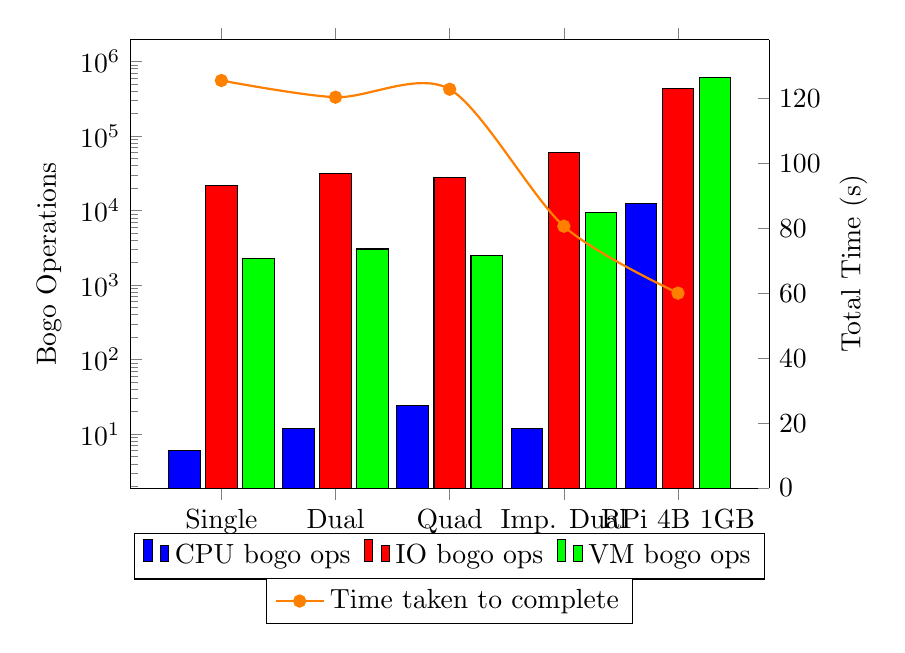
\begin{tikzpicture}
    \begin{axis}[
        width=0.8\textwidth,
        height=0.6\textwidth,
        ybar,
        bar width=0.4cm,
        enlarge x limits=0.2,
        legend style={
            at={(0.5, -0.1)},
            anchor=north,
            legend columns=-1,
            /tikz/every even column/.append style={column sep=0.1cm}
        },
        ylabel={Bogo Operations},
        symbolic x coords={Single, Dual, Quad, Imp. Dual, RPi 4B 1GB},
        xtick=data,
        axis y line*=left,
        ylabel near ticks,
        ymode=log,
        log origin=infty,
        ]
    \addplot[fill=blue] coordinates {
        (Single,6) (Dual,12) (Quad,24) (Imp. Dual, 12) (RPi 4B 1GB,12483)};
    \addplot[fill=red] coordinates {
        (Single,21794) (Dual,31190) (Quad,27819) (Imp. Dual,60868) (RPi 4B 1GB,440066)};
    \addplot[fill=green] coordinates {
        (Single,2280) (Dual,3053) (Quad,2464) (Imp. Dual,9552) (RPi 4B 1GB,617668)};
    \addlegendentry{CPU bogo ops}
    \addlegendentry{IO bogo ops}
    \addlegendentry{VM bogo ops}
    \end{axis}
    
    \begin{axis}[
        width=0.8\textwidth,
        height=0.6\textwidth,
        enlarge x limits=0.2,
        legend style={
            at={(0.5,-0.2)},
            anchor=north,
            legend columns=-1,
            /tikz/every even column/.append style={column sep=0.5cm}
        },
        axis y line*=right,
        axis x line=none,
        ylabel={Total Time (s)},
        ylabel near ticks,
        ymin=0,
        symbolic x coords={Single, Dual, Quad, Imp. Dual, RPi 4B 1GB},
        ]
    \addplot[smooth, thick, orange, mark=*] coordinates {
        (Single,125.45) (Dual,120.31) (Quad,122.76) (Imp. Dual,80.6) (RPi 4B 1GB,60.00)};
    \addlegendentry{Time taken to complete}
    \end{axis}
    \end{tikzpicture}
\end{figure*}

\newpage
\subsection{Results and Analysis}
\begin{table}[!ht]
    \centering
    \begin{tabular}{|l|l|l|l|l|}
    \hline
        Improved Dual Core Tests & Basic 1 & Basic 2 & Basic 3 & Large Scale 100 \\ \hline
        Total Bytes Processed (Mb) & 104.86 & 84.93 & 169.87 & 849.35 \\ \hline
        Avg Bytes per Second (Kb/s) & 376.04 & 406.06 & 393.59 & 403.36 \\ \hline
        Test Duration (s) & 278.85 & 209.17 & 431.59 & 2105.67 \\ \hline
        Total Network Time (s) & 51.08 & 71.65 & 108.20 & 646.95 \\ \hline
        Total Processing Time (s) & 227.77 & 137.52 & 323.39 & 1458.72 \\ \hline
        Avg Queue Time (s) & 0.08 & 3.11 & 1.95 & 2.81 \\ \hline
    \end{tabular}
    \caption{Dual Core Improved, Basic Test 2 Server Metrics}
    \label{Fig:2c-improved-server-metrics}
\end{table}

These optimisations translate directly to improved encryption performance. The improved design achieves throughput between 376-406 KB/s, approximately 50\% higher than the original dual core configuration. Processing times show similar improvement, with the Large Scale test completing in 2105.67s versus 3214.54s. Queue times reduce from 4.35s to 3.11s on average, suggesting better overall system responsiveness.

Operating temperature stabilizes slightly higher at 68-69°C, a modest increase that reflects the higher clock rate while remaining well within the Artix-7's thermal specifications. Interestingly, in the temperature plot for the improved dual core (Figure \ref{Fig:2c-improved-temperature}), once the air-conditioning in the lab was turned on, there was a gradual drop in temperature of one degree which was observed.

\begin{figure}[h!t]
    \begin{center}
        \caption{Raspberry Pi, Large Scale, 100 clients, Server Metrics}
        \label{Fig:2c-improved-temperature}
    \includegraphics[width=.7\textwidth]{Chapter4/Results/2c_improved_results/arty-a7-2c-improved_large_scale_1000_20241007_123418.db_server_temperature.png}
    \end{center}
\end{figure}

\section{Application Results Summary}

\begin{figure}[h]
    \centering
    \caption{Large Scale 100 Client Test Encryption Throughput Across Configurations}
    \label{fig:throughput-comparison}
    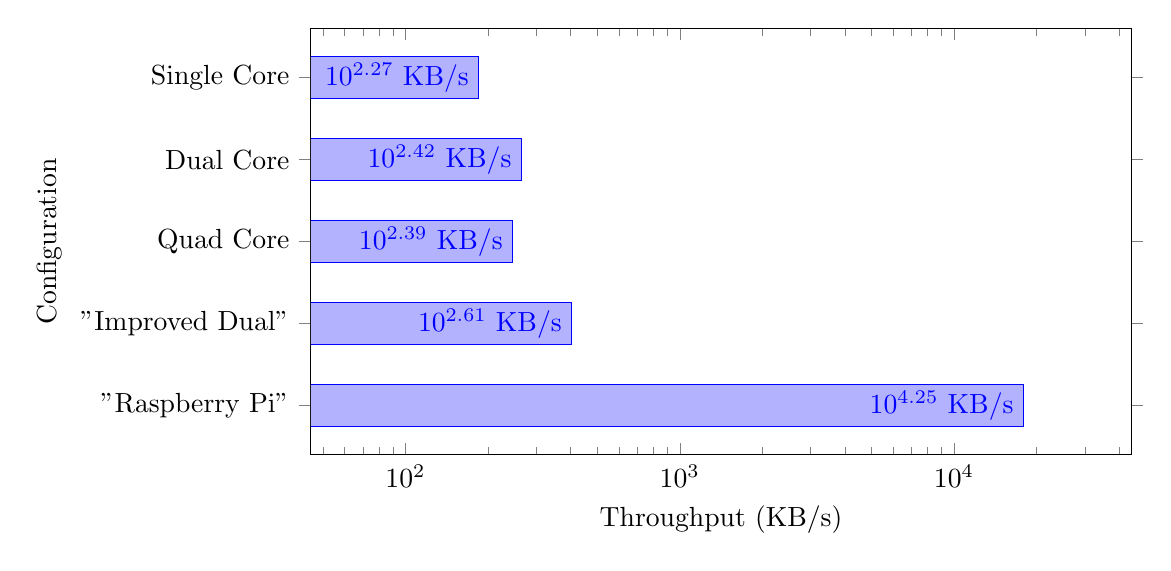
\begin{tikzpicture}
    \begin{semilogxaxis}[
        width=12cm,
        height=7cm,
        xbar,
        enlargelimits=0.15,
        xlabel={Throughput (KB/s)},
        ylabel={Configuration},
        symbolic y coords={Single Core,Dual Core,Quad Core,"Improved Dual","Raspberry Pi"},
        ytick=data,
        xmin=100,
        xmax=20000,
        log basis x=10,
        nodes near coords={$10^{\pgfmathprintnumber\pgfplotspointmeta}$ KB/s},
        nodes near coords align={left},
        bar width=15pt,
        y dir=reverse,
        fill=blue!40
    ]
    \addplot coordinates {
        (184.78,Single Core)
        (264.22,Dual Core)
        (245.57,Quad Core)
        (403.36,"Improved Dual")
        (17895.55,"Raspberry Pi")
    };
    \end{semilogxaxis}
    \end{tikzpicture}
    
\end{figure}

The performance analysis across configurations reveals clear trends in the viability of FPGA-based softcore processors for network security applications. Single core performance established a baseline of 221 KB/s maximum throughput, with dual core showing a 23\% improvement to 272 KB/s through effective parallel processing. The quad core configuration, however, demonstrated diminishing returns due to resource starvation, achieving only 269 KB/s despite doubled processing resources. The improved dual core design, implementing a 150MHz clock rate and quadrupled ethernet buffers, achieved the best FPGA performance at 406 KB/s - an 84\% improvement over the baseline.

However, these improvements still fall significantly short of the Raspberry Pi's 17,895 KB/s throughput, highlighting the performance gap between FPGA-based softcores and physical processor implementations. These results suggest that while FPGA softcore implementations can provide functional network security solutions, their performance remains fundamentally constrained by architectural and physical limitations.


\newpage
\section{Benchmarking TLS}
\label{section:TLS-benchmarking}
We will now observe how much overhead is introduced by running the full TLS1.3 stack on the SCPNS. We will begin by generating the key and the certificates using a 2048-bit RSA:
\begin{verbatim}
    openssl req -x509 -newkey rsa:2048 -keyout key.pem -out cert.pem -days 365
-nodes
\end{verbatim}
This process took roughly two minutes, whereas on hardcore processors, such as the Raspberry Pi, it is instant. Next, we need to start a server on the SCPNS running TLS1.3. Forunately, OpenSSL also has testing utilities for this scenario. We can start a server using our newly generated key and certificate:
\begin{verbatim}
    openssl s_server -cert cert.pem -key key.pem -accept 8443 -cipher 
AES256-GCM-SHA256
\end{verbatim}

From a client device, such as the Raspberry Pi, we can also use OpenSSL to act as a client and begin a TLS1.3 end-to-end encrypted stream via:
\begin{verbatim}
    dd if=/dev/zero bs=1K count=64 2>/dev/null | \
        openssl s_client -connect 192:168.1.50:8443 \
        -cipher AES256-GCM-SHA256 2>/dev/null | \
        dd of=/dev/null 2>/dev/null
\end{verbatim}

The surrounding `\texttt{dd}' commands specify the size of the message to send, in this case it is 64KB. To get a comprehensive overview, we will run streams of sizes: 64KB, 128KB, 256KB, 512KB and 1024KB; each three times to get an average throughput. Table \ref{TLS1.3Benchmark} shows the results.

\begin{table}[!ht]
    \centering
    \begin{tabular}{l|ll|l}
    \textbf{\begin{tabular}[c]{@{}l@{}}Stream Size\\ (KB)\end{tabular}} & \textbf{\begin{tabular}[c]{@{}l@{}}(No HW) AES\\ (KB/s)\end{tabular}} & \textbf{\begin{tabular}[c]{@{}l@{}}(HW) AES\\ (KB/s)\end{tabular}} & \textbf{Difference}             \\ \hline
    64        & 20.44                                                                 & 19.22    & {\color[HTML]{FE0000} -5.97\%}  \\
    128       & 12.76                                                                 & 13.24    & {\color[HTML]{32CB00} +3.76\%}  \\
    256       & 12.80       & 12.80    & 0\%                             \\
    512       & 14.90       & 13.24    & {\color[HTML]{FE0000} -11.14\%} \\
    1024      & 13.70       & 13.75    & {\color[HTML]{32CB00} +0.36\%} 
    \end{tabular}
    \caption{TLS1.3 Benchmark on the SCPNS, AES256-GCM-SHA256 Cipher, Results}
    \label{TLS1.3Benchmark}
\end{table}

Disappointingly, these benchmarks reveal that the hardware acceleration of AES operations on the SCPNS had minimal impact on overall throughput. Across the different stream sizes the performance differences between hardware and software implementations ranged from -11.14\% to +3.76\%, with some sizes showing negligible change. Despite the 4x improvement seen in raw AES benchmarks, these gains did not translate to TLS performance, suggesting that the bottleneck lies elsewhere in the protocol stack - likely in the TLS overhead (handshake, key exchange, \etc), network interface, or memory subsystem rather than in the cryptographic operations themselves. Observe as well, that our raw TCP throughput for the improved dual core was 21.6Mbits/s  (Table \ref{table:ethernet2}). By running TLS1.3, the throughput is significantly reduced to 12-20KB/s.

\newpage
\section{Utilisation of Configurations}
Analysis of FPGA resource utilisation across configurations reveals how the design scales with additional cores and improvements:

\textbf{Logic Resources (LUTs and FFs):}
\begin{itemize}
    \item Single core uses 41.24\% of available LUTs and 19.05\% of FFs.
    \item Dual core increases to 60.19\% LUTs and 27.25\% FFs.
    \item Quad core reaches 94.13\% LUTs and 40.73\% FFs.
    \item Improved dual core uses 89.81\% LUTs and 28.45\% FFs.
\end{itemize}

The near-linear scaling in register usage (roughly +8\% FFs per core) suggests efficient core replication. However, LUT utilisation shows diminishing returns, with the quad-core configuration nearly maxing out the device's logic resources. This solidifies why we could not further optimise the quad-core configuration - there weren't any resources left.

\textbf{Memory Resources:}
\begin{itemize}
    \item BRAM utilisation scales from 74\% (single) to 83\% (dual) to 99\% (quad).
    \item The improved dual core uses 100\% of available BRAM, mainly due to enlarged buffers.
    \item This indicates memory resources become a limiting factor for further optimisation.
\end{itemize}

\textbf{DSP Usage:}
\begin{itemize}
    \item DSP utilisation scales linearly with core count (4, 8, and 16 DSPs respectively).
    \item Only using up to 17.78\% of available DSP resources.
    \item DSPs are primarily used for address generation and memory management.
\end{itemize}

The improved dual-core design, while using similar FF resources to the standard dual-core, shows significantly higher LUT and BRAM usage due to its increased amount of buffers for ethernet and interconnects. This represents a better balance of resource utilisation versus performance, as demonstrated by the throughput results (Table \ref{table:ethernet2}). The full utilisation of the improved dual core can be seen in table \ref{table:imp-2c-util}.

\begin{table}[!ht]
    \centering
    \begin{tabular}{llll}
    \textbf{Resource Type}                              & \textbf{Used} & \textbf{Available} & \textbf{Utilisation} \\ \hline
    \multicolumn{1}{l|}{\textbf{Slice LUTs}}            & 18,680        & 20,800             & 89.81\%              \\
    \multicolumn{1}{l|}{\textbf{- LUT as Logic}}        & 15,124        & 20,800             & 72.71\%              \\
    \multicolumn{1}{l|}{\textbf{- LUT as Memory}}       & 3,556         & 9,600              & 37.04\%              \\
    \multicolumn{1}{l|}{\textbf{Slice Registers (FFs)}} & 11,836        & 41,600             & 28.45\%              \\
    \multicolumn{1}{l|}{\textbf{Block RAM Tiles}}       & 50            & 50                 & 100.00\%             \\
    \multicolumn{1}{l|}{\textbf{- RAMB36}}              & 42            & 50                 & 84.00\%              \\
    \multicolumn{1}{l|}{\textbf{- RAMB18}}              & 16            & 100                & 16.00\%              \\
    \multicolumn{1}{l|}{\textbf{DSPs}}                  & 8             & 90                 & 8.89\%              
    \end{tabular}
    \caption{Improved Dual Core Utilisation}
    \label{table:imp-2c-util}
    \end{table}

\newpage
\section{Timing Analysis}
\label{section:timing-analysis}
The timing analysis reveals critical path constraints that limit our system's maximum operating frequency. While all configurations are stable at 100MHz, attempts to increase the clock rate to 150MHz expose several timing violations:

\textbf{Critical Paths:}

Our most significant timing violations occur in the DDR3 memory interface, with:
\begin{itemize}
    \item Worst Negative Slack (WNS): -2.805ns
    \item Total Negative Slack (TNS): -9230.256ns
    \item 11,401 failing endpoints out of 57,626 total endpoints
\end{itemize}

Figure \ref{pathfails}, shows the majority of these failed paths are attached to the `\texttt{main\_crg\_clkout0}' clock domain.

\begin{figure}[!ht]
    \begin{center}
        \includegraphics[width=1\textwidth]{Chapter4/Figures/462581922_574957911686367_780340784793017917_n.png}
    \end{center}
    \caption{Critical Path Failures W.R.T \texttt{main\_crg\_clkout0}}
    \label{pathfails}
\end{figure}

These violations center around in the DDR3 controller interface where tight timing requirements exist for address and control signals. The negative slack of -2.805ns indicates we're missing our timing requirements by approximately 3 nanoseconds on the worst paths. However, despite these failed paths, we were still able to complete the full test suite at 150MHz. Presumably, there must be a sufficient error margin in the DDR3 protocol to accommodate this timing uncertainty.

This analysis suggests that to achieve a higher clock rate on the Digilent Arty A7, the memory controller path from the VexRiscvSMP should be optimised first, however, this is out of scope for this thesis.

\newpage
\section{Power Usage Analysis}
\label{section:PowerAnalysis}
Power consumption was analysed both theoretically through Vivado's power analysis and through real-world measurements using the board's XADC (see XADC in Digilent Reference Manual \cite{ArtyA7RefManual}).

\begin{wrapfigure}[16]{l}{0.6\textwidth}
    \centering
    \caption{Synthesis With AES Instructions Power Report.}
    \label{PowerReports}
    \includegraphics[width=0.6\textwidth]{Chapter4/Figures/power-with-aes.png}
    \caption{Synthesis Without AES instructions Power Report.}
    \label{AESPowerReport}
    \includegraphics[width=0.6\textwidth]{Chapter4/Figures/power-no-aes.png}
\end{wrapfigure}

Core power consumption was evaluated both with and without custom AES instructions:

\begin{itemize}
    \item Without AES instructions: 0.935W.
    \item With AES instructions: 0.944W.
    \item Power overhead of AES: $\sim$9mW (0.96\% increase).
\end{itemize}
The AES-enabled configuration power is distributed across:

\begin{itemize}
    \item Dynamic Power: 0.876W (93\%).
    \item I/O: 0.213W (24\%).
    \item BRAM: 0.175W (20\%).
    \item Signals: 0.127W (14\%).
    \item Clocks: 0.084W (10\%).
    \item Other (PLLs, MMCM, \etc): $\sim$0.277W (25\%).
    \item Static Power: 0.068W (7\%).
\end{itemize}

The PLL and MMCM can be disabled if power needs to be reduced more, as we do not use these components in the application. Furthermore, the total power used by the FPGA core was confirmed by reading the \texttt{VCCINT} register on the XADC.

Real-world measurements through the XADC's \texttt{VCCAUX} register show a total board power consumption of 1.77W. This higher figure accounts for all board components, FPGA core (0.944W), DDR3 memory module, Ethernet PHY, Voltage regulators and clock generators as well as the LEDs.

The total power consumption of 1.77W, while modest for a full-featured network security processor, is still significant for battery-powered or ultra-low-power applications. The FPGA maintains this power draw even when idle, as the design lacks power-saving states or clock gating mechanisms. Typically, this is solved by implementing a low power co-microcontroller to manage FPGA power states, \ie power gating circuitry to completely disable the FPGA when not needed and a boot management system to quickly restore the FPGA state when encryption services are required.

